\documentclass[
    a4paper
]{scrreprt}
\usepackage[ngerman]{babel}
\usepackage[utf8]{inputenc}
\usepackage{textcomp, expdlist, array, colortbl, xcolor}
%\usepackage{wrapfig}
\usepackage[pdftex]{graphicx}
\usepackage[TS1, T1]{fontenc}
\usepackage{palatino} % Schriftart
\usepackage{parskip} %Erste Zeile eines Paragrafen nicht einrücken

\usepackage{listings}
\usepackage{color}
\usepackage{xcolor}

\colorlet{punct}{red!60!black}
\definecolor{background}{HTML}{EEEEEE}
\definecolor{delim}{RGB}{20,105,176}
\colorlet{numb}{magenta!60!black}
\definecolor{mygreen}{rgb}{0,0.6,0}

\lstdefinelanguage{json}{
	basicstyle=\normalfont\ttfamily,
	stepnumber=1,
	numbersep=8pt,
	showstringspaces=false,
	breaklines=true,
	backgroundcolor=\color{background},
	morestring=[s][\color{red}]{"}{"},
	morekeywords={set, hash, key},
	morecomment=[l]{//},
	literate=
	*{0}{{{\color{numb}0}}}{1}
	{1}{{{\color{numb}1}}}{1}
	{2}{{{\color{numb}2}}}{1}
	{3}{{{\color{numb}3}}}{1}
	{4}{{{\color{numb}4}}}{1}
	{5}{{{\color{numb}5}}}{1}
	{6}{{{\color{numb}6}}}{1}
	{7}{{{\color{numb}7}}}{1}
	{8}{{{\color{numb}8}}}{1}
	{9}{{{\color{numb}9}}}{1}
	{:}{{{\color{punct}{:}}}}{1}
	{,}{{{\color{punct}{,}}}}{1}
	{\{}{{{\color{delim}{\{}}}}{1}
	{\}}{{{\color{delim}{\}}}}}{1}
	{[}{{{\color{delim}{[}}}}{1}
	{]}{{{\color{delim}{]}}}}{1}
	{1aba56d8c5}{{{\color{numb}1aba56d8c5}}}{10}
}

\lstset{
	language={json},
	commentstyle=\color{mygreen}
}	
	
	
\begin{document}
    \sffamily % Whole document sans-serif


    % Titelseite
    \begin{titlepage}
        \centering
        
\includegraphics[width=0.8\textwidth]{./images/logo_hska.png}\par\vspace{1cm}
        \vspace{1cm}

        {\scshape\Large Verteile Systeme 2 -- Labor\par}
        \vspace{1.5cm}

        {\huge\textbf{Twitter-Klon}\par}
        \vspace{2cm}

        {\Large\itshape Timo Blust, 48594\par}
        {\Large\itshape Gennadi Eirich, 50629\par}
        {\Large\itshape Tim Essig, 49683\par}
        {\Large\itshape Maike Rees, 47307\par}
        
        \vfill

        % Bottom of the page
        {\large \today\par}
    \end{titlepage}


    % Inhaltsverzeichnis
    \tableofcontents


    % Aufgabe 1
    \chapter{Konzeption und Gestaltung}
    \section{Use Case Diagramm}
    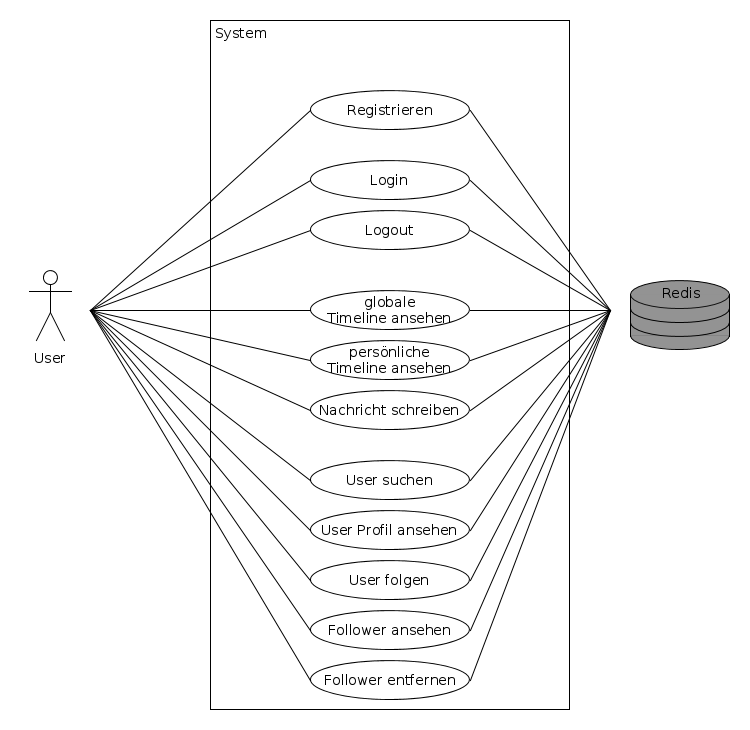
\includegraphics[width=\textwidth]{./images/useCaseDiagramm.png}
    \section{Entwurf der Seitennavigation}
    
    \section{Mockup}
		\includegraphics[width=\textwidth]{./images/1_login.png}
		Login\par\vspace{.6cm}
		\includegraphics[width=\textwidth]{./images/1_registration.png}
		Registration\par\vspace{.6cm}
		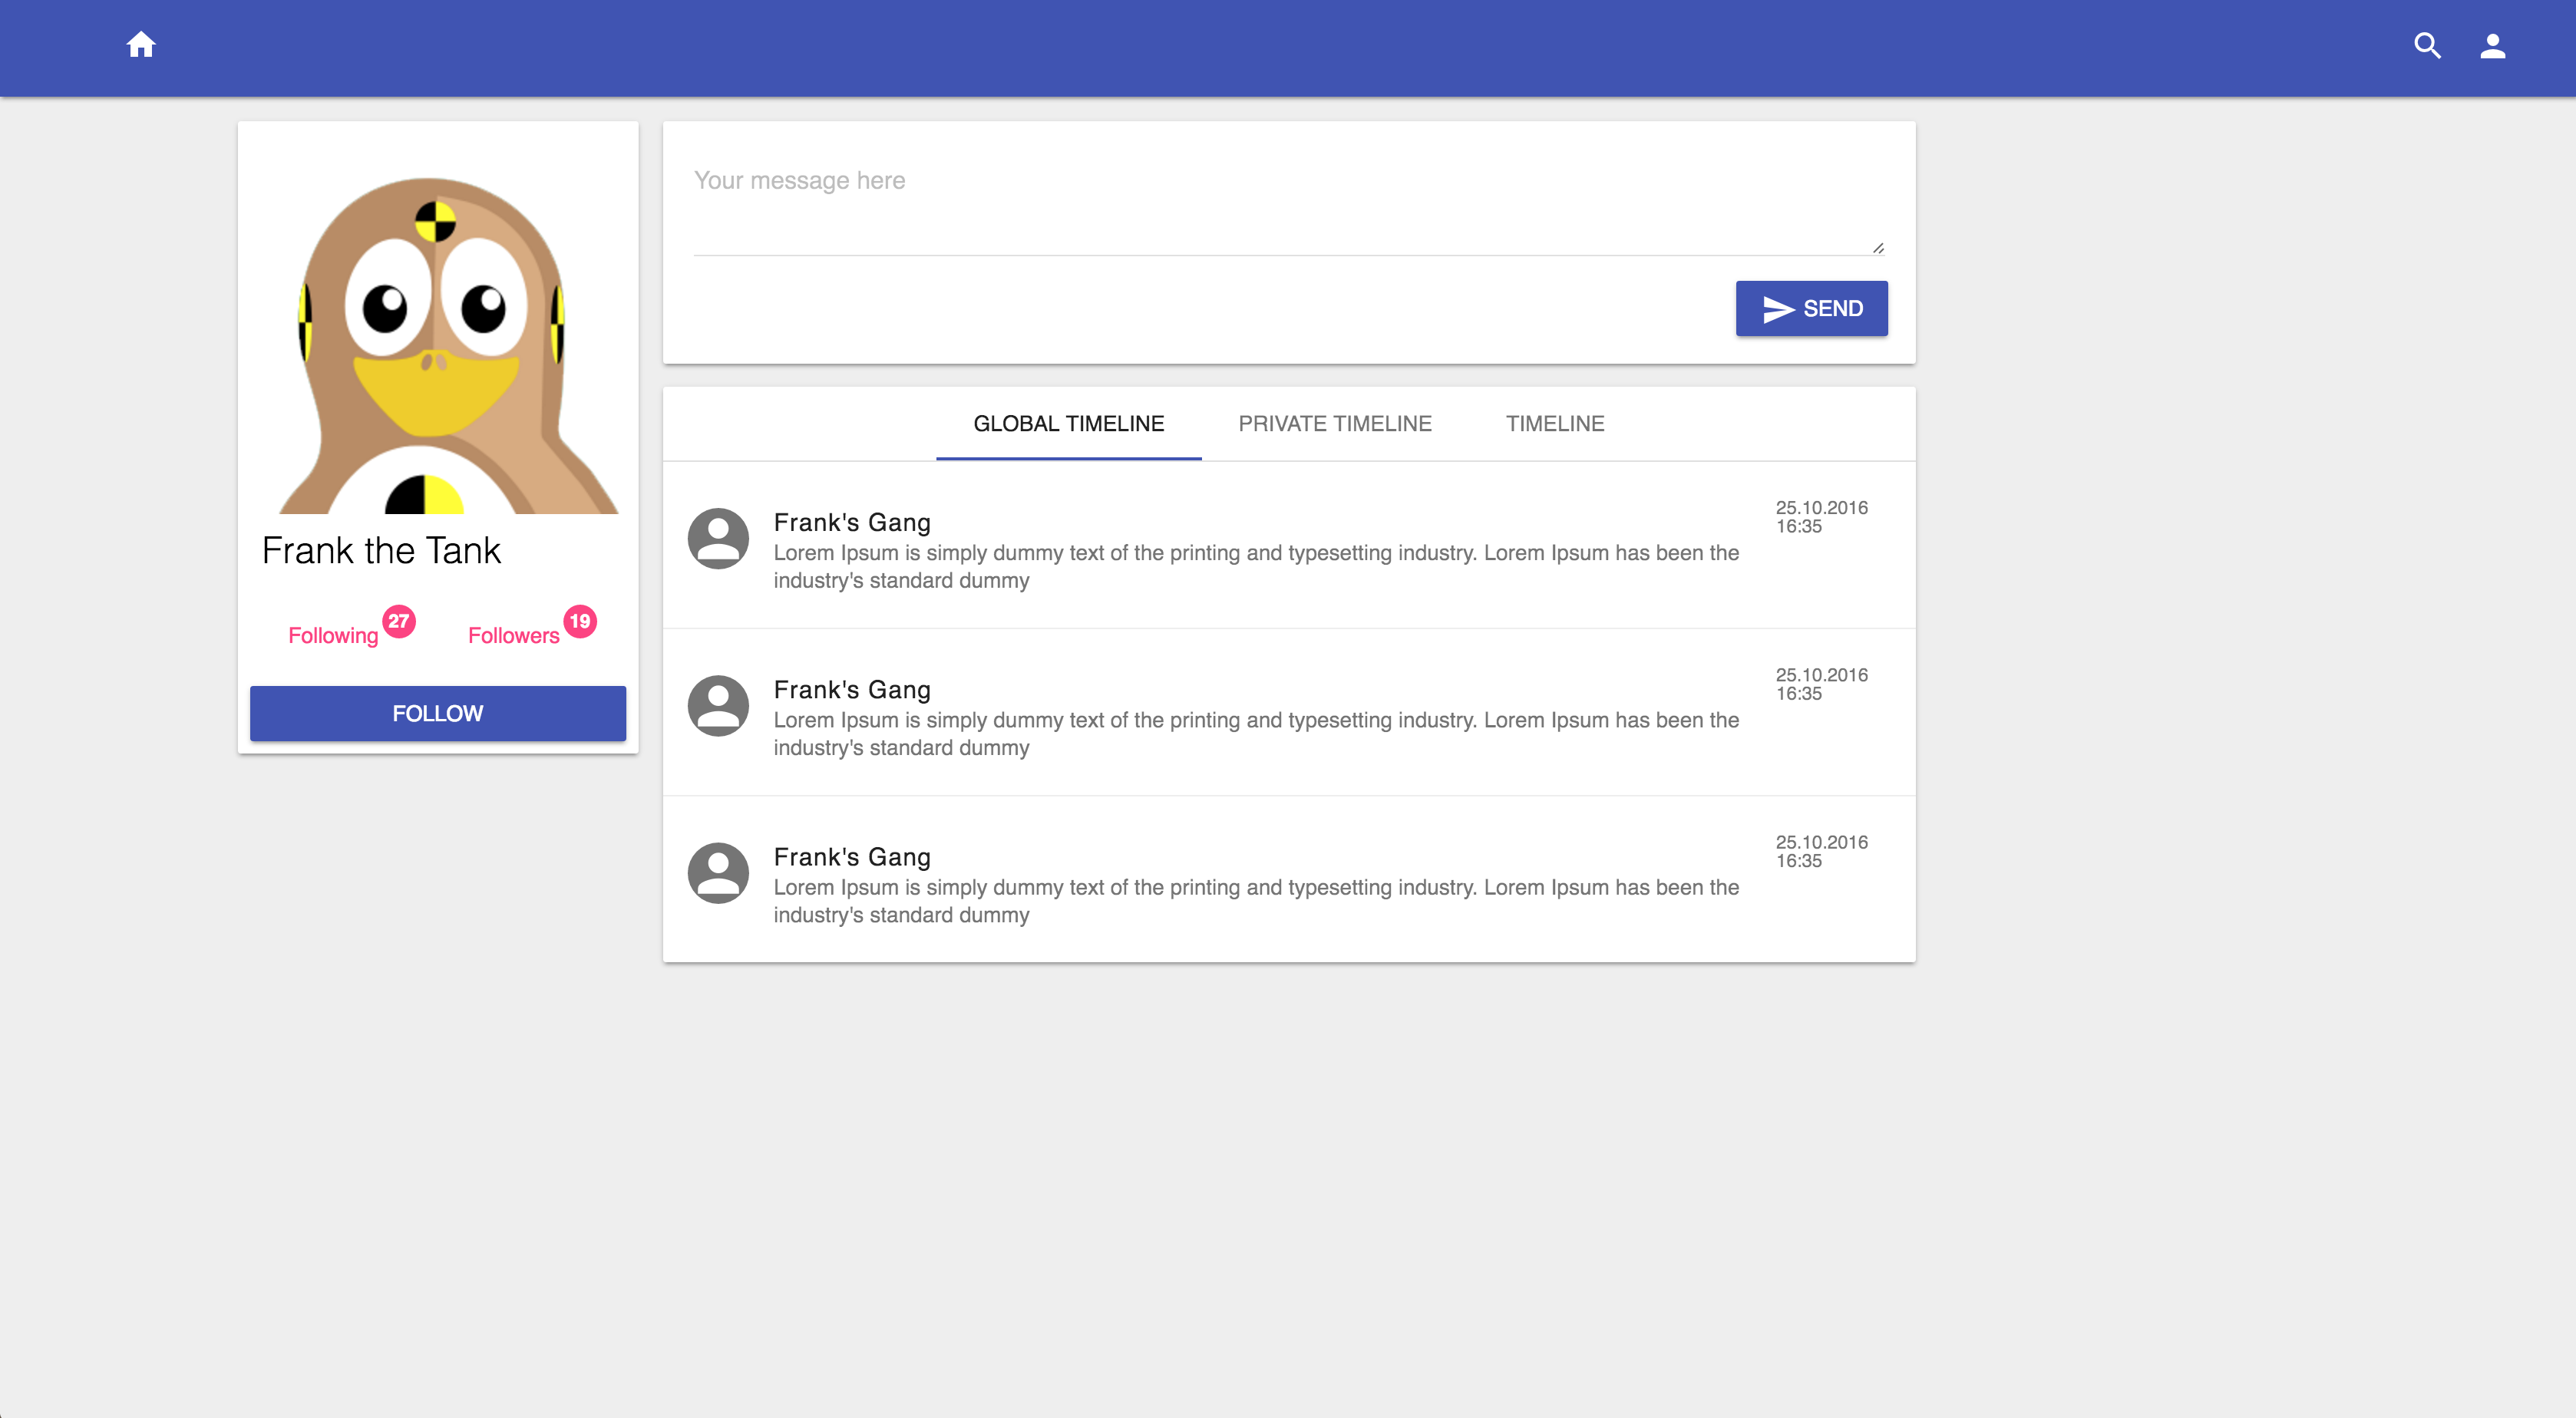
\includegraphics[width=\textwidth]{./images/1_home.png}
		Home\par\vspace{.6cm}
		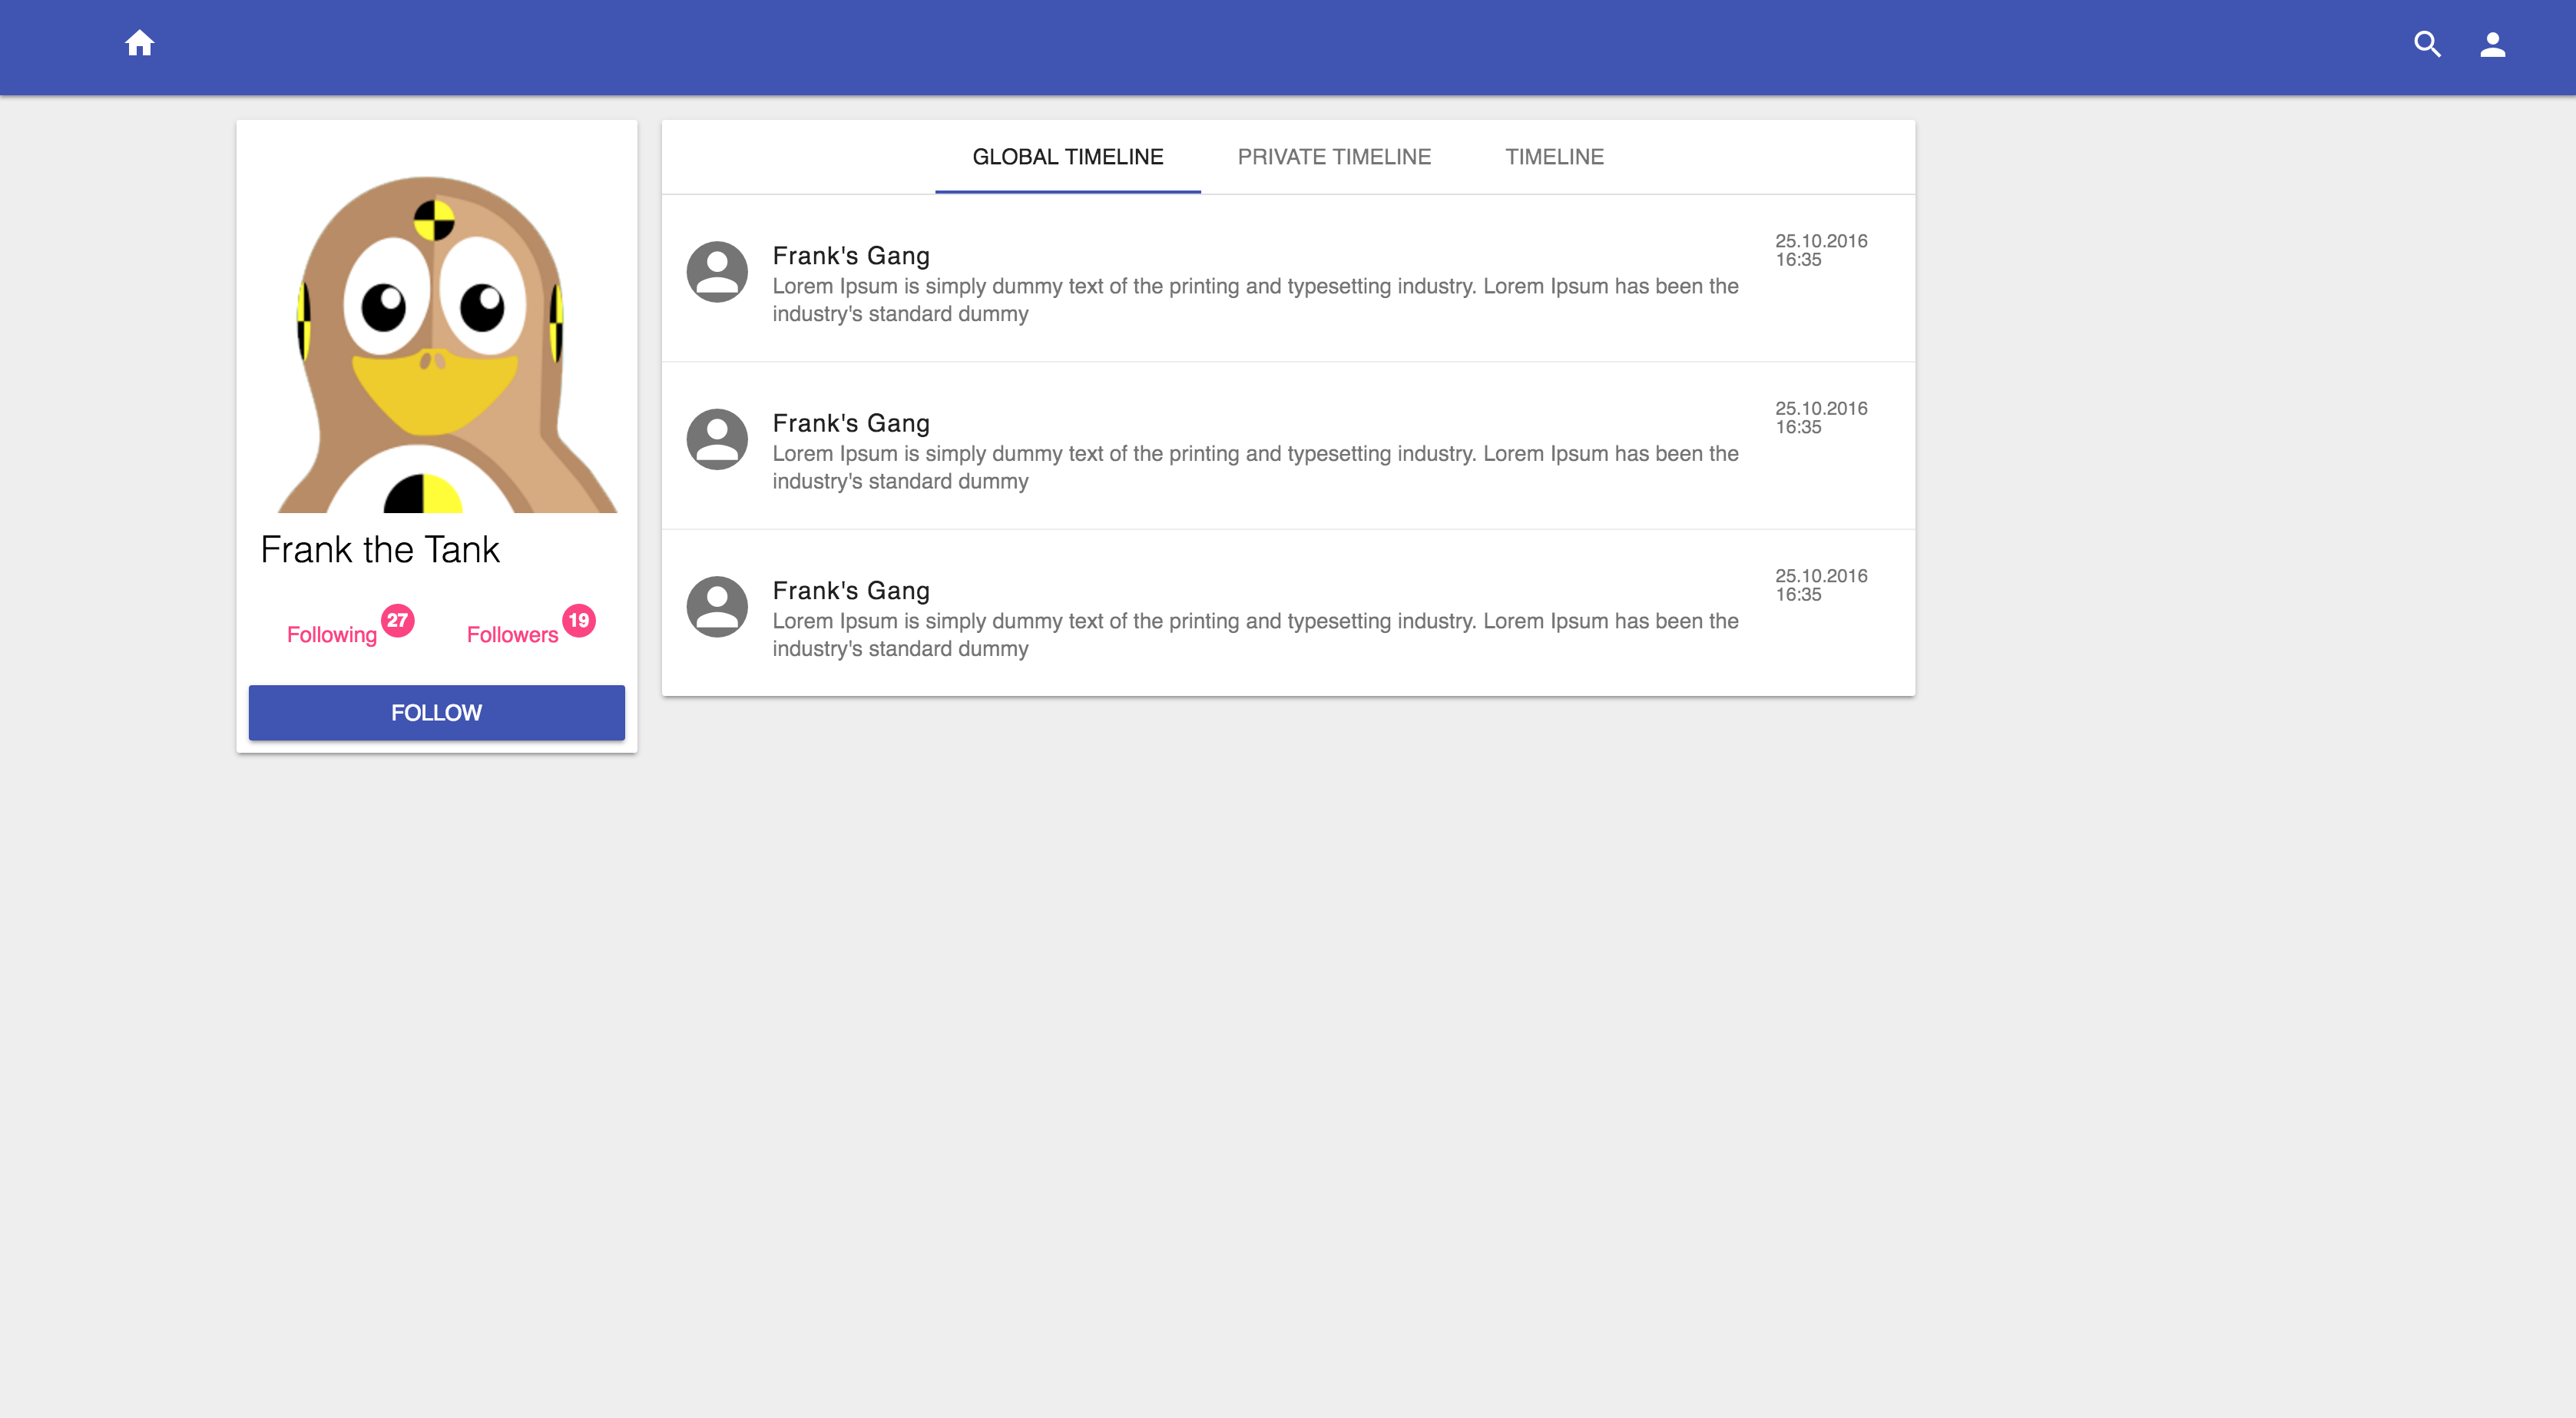
\includegraphics[width=\textwidth]{./images/1_user.png}
		Benutzeransicht\par\vspace{.6cm}
		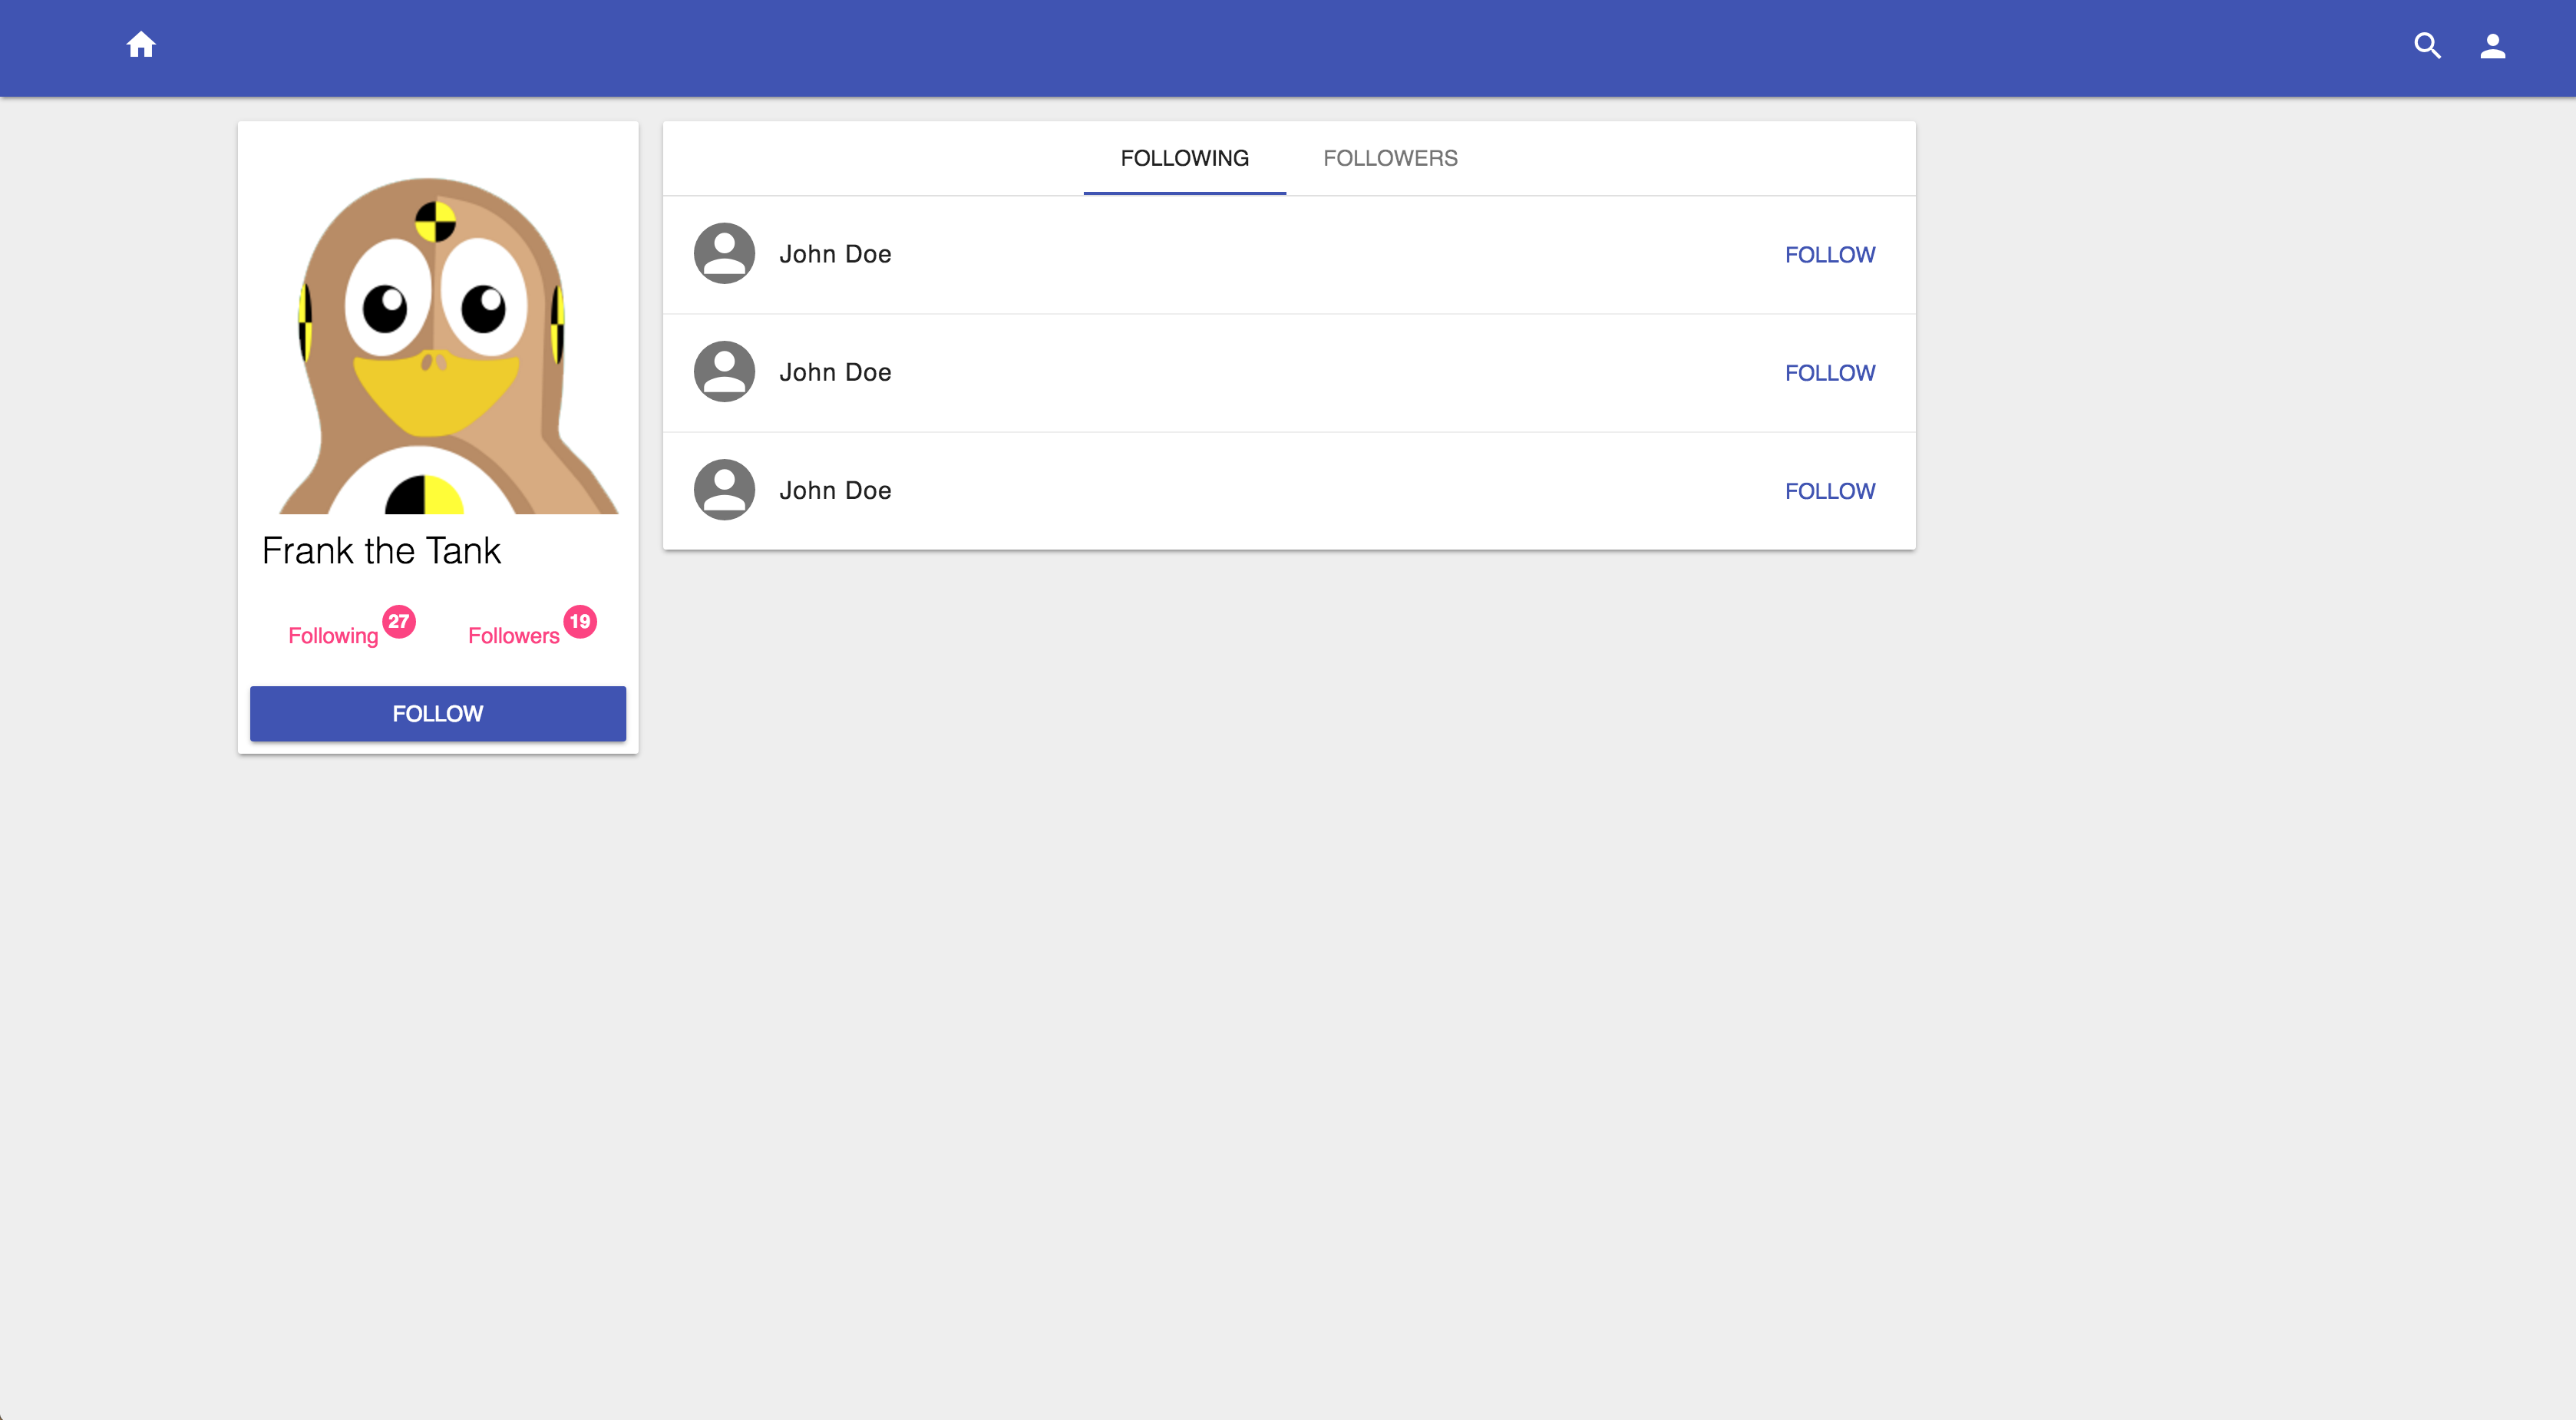
\includegraphics[width=\textwidth]{./images/1_user_followers.png}
		Followerliste des Benutzers
    
%   \section{Datenmodell}
%    
%    \subsection*{Globale Zähler}
%		\begin{enumerate}
%			\item \textit{next\_user\_id} {Zähler für die nächste zu vergebende User ID}
%			\item \textit{next\_post\_id} {Zähler für die nächste zu vergebende Post ID}
%		\end{enumerate}
%	
%	\subsection*{Users}
%		Für die User wird eine HashMap angelegt, die dem Namensschema \textit{user:[user\_id]} folgt. %Die nächste ID bekommt man über \textit{INCR next\_user\_id}. \\
%		Die HashMap hat folgende Felder:
%		\begin{enumerate}
%			\item \textit{username} {Der Name des Users}
%			\item \textit{password} {Das Passwort des Users(hashed + salted)}
%			\item \textit{auth} {Authentifizierungs-Token des Nutzers}			
%		\end{enumerate}
%		
%		Wenn ein User angelegt wird, so muss dessen ID in dem HashSet \textit{users} hinzugefügt werden, z.B: \textit{HSET users essigt 1000}\\
%		
%		Zudem muss der Authentifizierungs-Token des Nutzers mit der User-ID verknüpft werden, dies wird in dem HashSet \textit{auths} hinterlegt. \\
%		
%		Um zu speichern, wem der User folgt, bzw. von wem er gefolgt wird, werden pro User zwei Sets benötigt:
%		\begin{enumerate}
%			\item followers:1000 {Die User-IDs die dem Benutzer 1000 folgen}
%			\item following:1000 {Die User-IDs denen der Benutzer 1000 folgt}
%		\end{enumerate}
%
%	
%	\subsection*{Posts}
%		Für die Posts wird eine HashMap angelegt, die dem Namensschema \textit{post:[post\_id]} folgt. Die nächste ID bekommt man über \textit{INCR next\_post\_id}. \\
%		Die HashMap hat folgende Felder:
%		\begin{enumerate}
%			\item \textit{user\_id} {Die User-ID des Erstellers}
%			\item \textit{timestamp} {Der Zeitstempel im Unix-Zeitformat}
%			\item \textit{message} {Der Text des Posts}
%		\end{enumerate}
%		
%		Wenn ein neuer Post angelegt wird, muss dessen ID in die Liste \textit{posts} hinzugefügt werden. Beispiel: \textit{ LPUSH [post\_id]} \\
%		Zudem muss der Post zu jeder Timeline der Follower und zu der Timeline des Erstellers hinzugefügt werden.
%		Für jeden User gibt es daher eine Liste \textit{timeline:[user\_id]}.
		
		\section{Datenmodell}

		
		\begin{lstlisting}[language=json]
//Set aller User
set user:all = {"essigt", "eirichg", "reesm", "blustt"}

//HashSets fuer die einzelnen Nutzer
hash user:*
	user:essigt = {id: "1", username: "essigt", firstname: "Tim", lastname: "Essig", password: "xyz", auth: "1aba56d8c5"}

//Sets um zu speichern, wer wem folgt
set user:*:follower
set user:*:following

//Keys um einen auth-token einem username zuzuordnen
key auth:*:username
	auth:1aba56d8c5:username = essigt

//Set aller Posts
set post:all = {1,2,3,4}

//HashSets fuer die einzelnen Posts
hash post:*
	post:1 = {timestamp: 01-03-2016 13:37, message:"Meine tolle Nachricht", user:"essigt"}

list user:*:posts = {1} //Liste aller Posts eines Users
list timeline:* = {1,3} //Liste aller Posts der Follower des Users(incl. seiner eigenen)

//Globale Counter
key global:userid
key global:postid
		\end{lstlisting}
	

    % Aufgabe 2
%    \chapter{Seitenbasierte Implementierung}


    % Aufgabe 3
%    \chapter{Asynchrone Erweiterungen}


\end{document}